\chapter{Some extra stuff}
\label{AppendixA}

\section{Marginal Abatement Cost Curve}
\label{sec:MACC}


\section{Financial Predictors Full-Size Graphs}
\label{sec:FinancialPreds}

\begin{figure}[H]
\centering
\subcaptionbox{Total Assets\label{fig:total-assets}}{%
  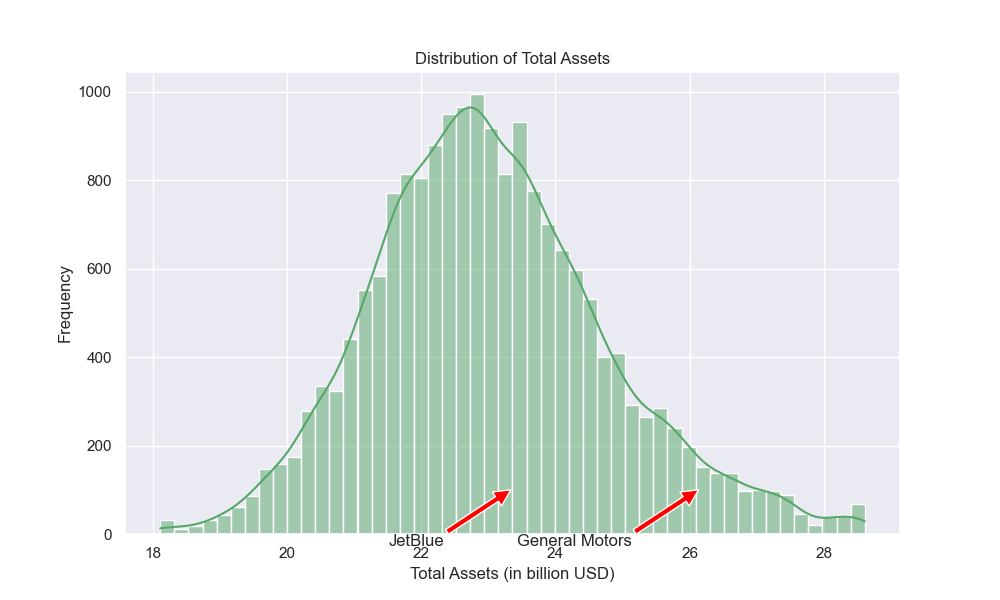
\includegraphics[width=0.8\textwidth]{figures/financial_preds/tot_assets_dist.png}}
\caption{Financial Predictors: Total Assets}
\end{figure}

\begin{figure}[H]
\centering
\subcaptionbox{Market Capitalization\label{fig:market-capitalization}}{%
  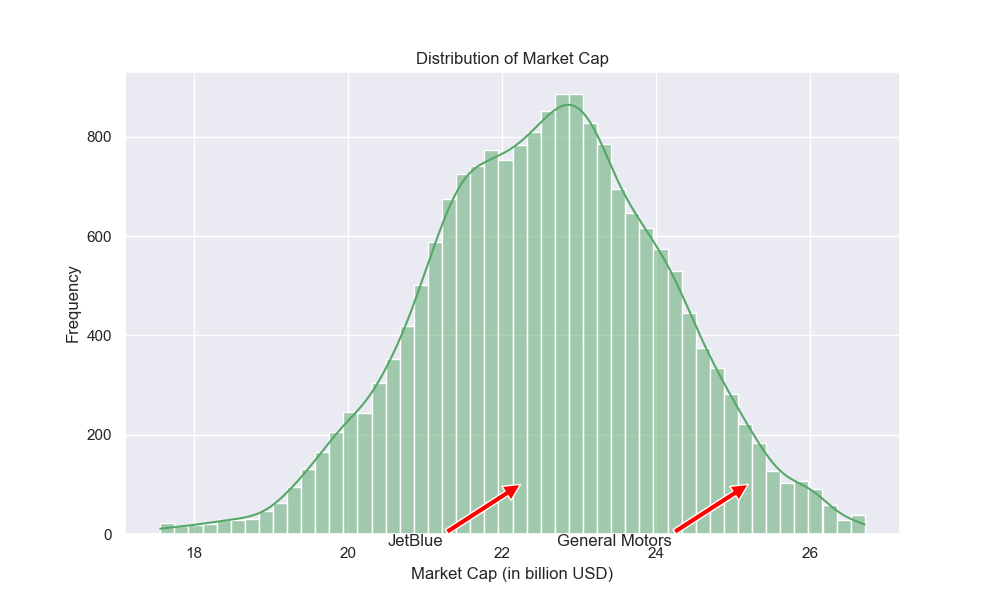
\includegraphics[width=0.8\textwidth]{figures/financial_preds/mkt_cap_dist.png}}
\caption{Financial Predictors: Market Capitalization}
\end{figure}

\begin{figure}[H]
\centering
\subcaptionbox{Return on Equity\label{fig:roe}}{%
  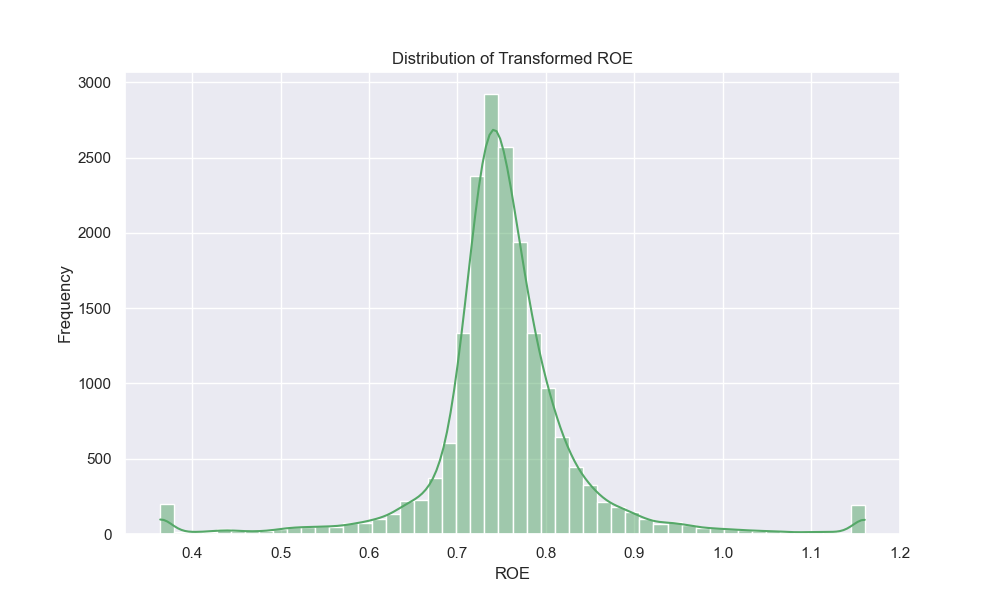
\includegraphics[width=0.8\textwidth]{figures/financial_preds/roe_dist.png}}
\caption{Financial Predictors: Return on Equity}
\end{figure}

\begin{figure}[H]
\centering
\subcaptionbox{Revenue\label{fig:revenue}}{%
  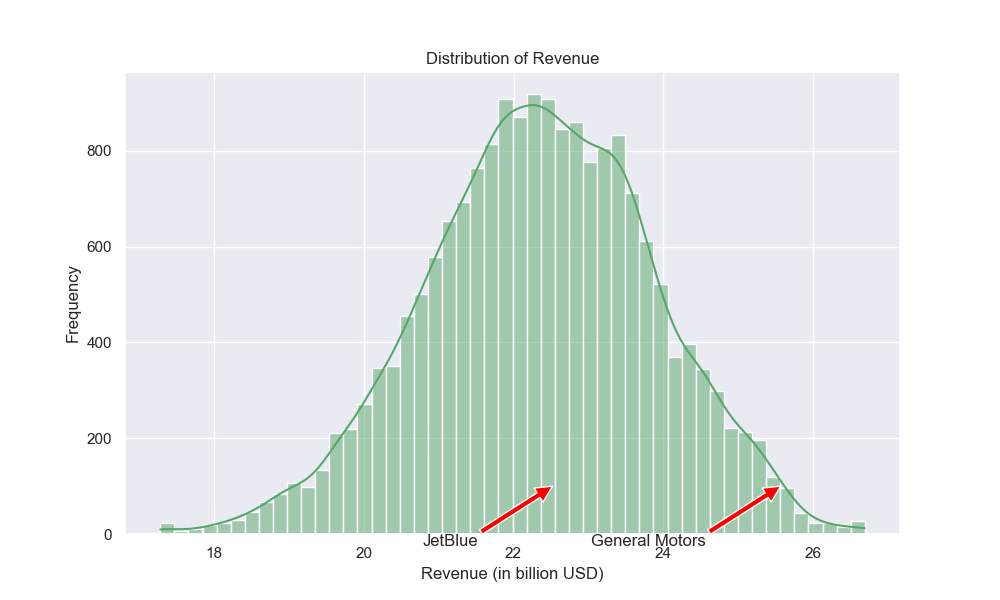
\includegraphics[width=0.8\textwidth]{figures/financial_preds/revenue_dist.png}}
\caption{Financial Predictors: Revenue}
\end{figure}

\begin{figure}[H]
\centering
\subcaptionbox{Net Income\label{fig:net-income}}{%
  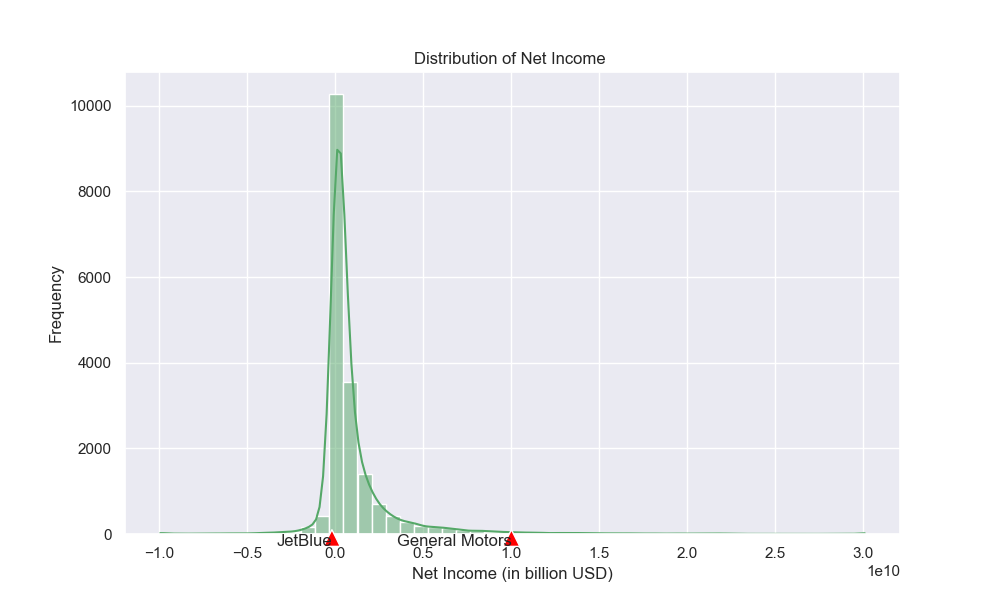
\includegraphics[width=0.8\textwidth]{figures/financial_preds/net_income_dist.png}}
\caption{Financial Predictors: Net Income}
\end{figure}

\begin{figure}[H]
\centering
\subcaptionbox{Employees\label{fig:employees}}{%
  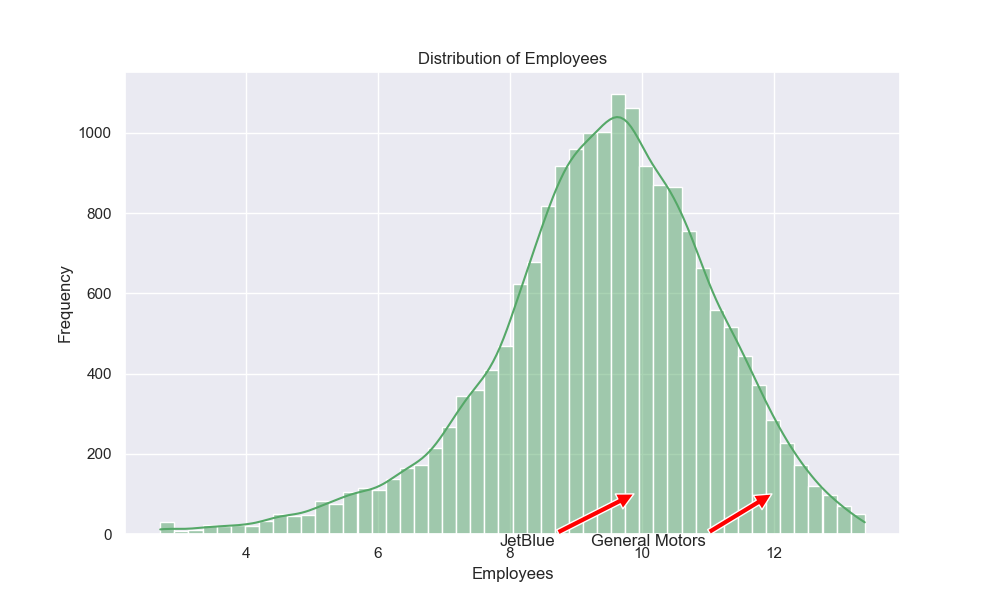
\includegraphics[width=0.8\textwidth]{figures/financial_preds/employees_dist.png}}
\caption{Financial Predictors: Employees}
\end{figure}

\begin{figure}[H]
\centering
\subcaptionbox{Total Assets 1yr Growth\label{fig:total-assets-1yr-growth}}{%
  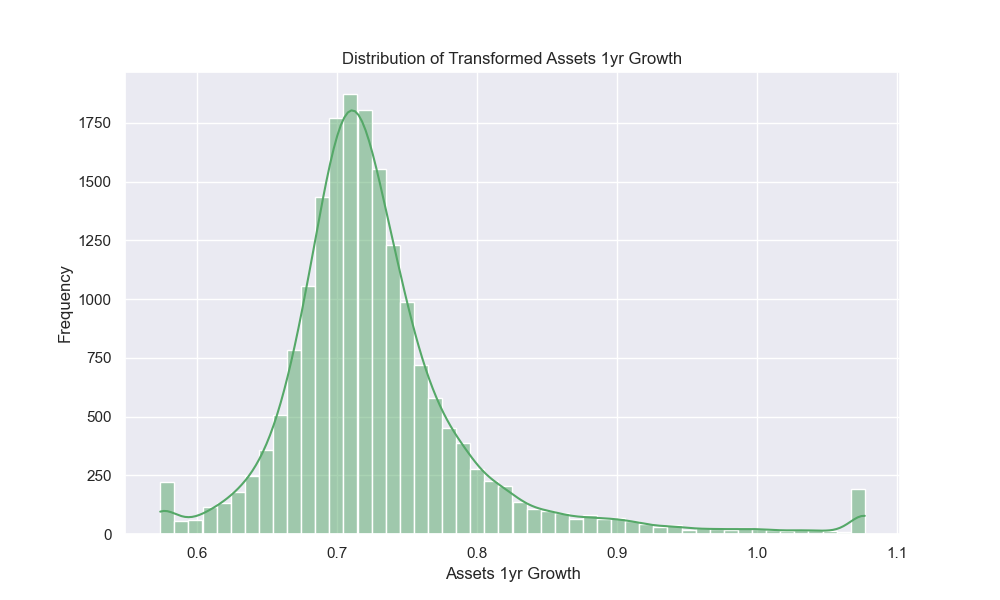
\includegraphics[width=0.8\textwidth]{figures/financial_preds/assets_1yr_growth_dist.png}}
\caption{Financial Predictors: Total Assets 1yr Growth}
\end{figure}

\begin{figure}[H]
\centering
\subcaptionbox{Employees 1yr Growth\label{fig:employees-1yr-growth}}{%
  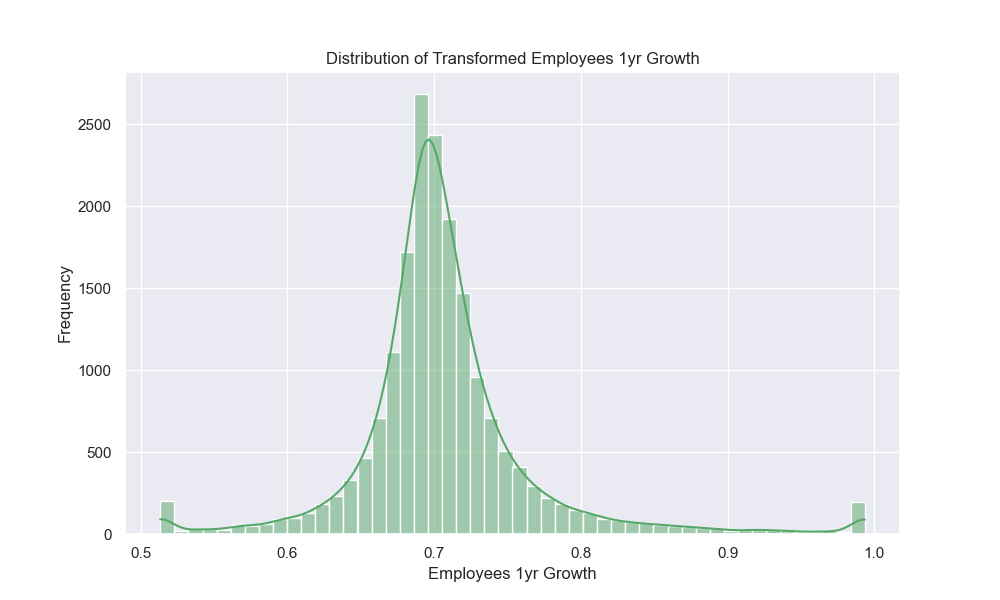
\includegraphics[width=0.8\textwidth]{figures/financial_preds/employees_1yr_growth_dist.png}}
\caption{Financial Predictors: Employees 1yr Growth}
\end{figure}

\begin{figure}[H]
\centering
\subcaptionbox{Net Income Over Assets\label{fig:net-income-over-assets}}{%
  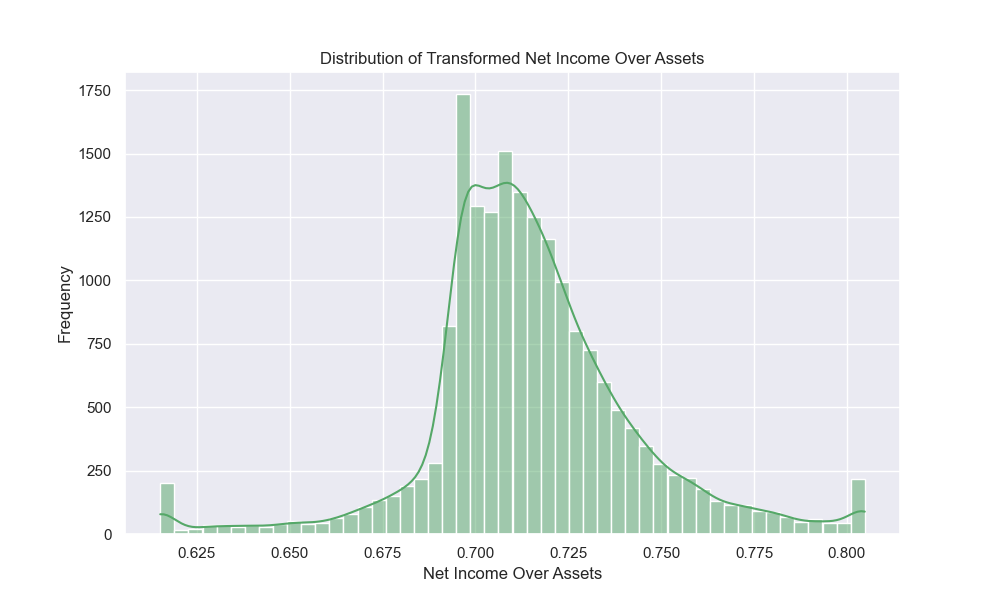
\includegraphics[width=0.8\textwidth]{figures/financial_preds/net_income_over_assets_dist.png}}
\caption{Financial Predictors: Net Income Over Assets}
\end{figure}


%  \setlength{\tabcolsep}{4pt}
%  \renewcommand{\arraystretch}{2.4}
% \footnotesize
% \begin{center}
%   \begin{tabular}{lcccc}
%     \hline
%  \textbf{Name} & \textbf{Param.} & \textbf{PMF or PDF} & \textbf{Mean} & \textbf{Variance} \\ 
%     \hline
%     Bernoulli & $p$ & $P(X=1) =p, P(X=0) = q$ & $p$ & $pq$ \\ 
%     Binomial & $n,p$ & ${n \choose k} p^k q^{n-k},   \,k \in \{0,1,\dots,n\}$ & $np$ & $npq$\\ 
%     FS & $p$ & $pq^{k-1},  \,k \in \{1,2,\dots\}$& $1/p$ & $q/p^2$\\ 
%     Geom & $p$ & $pq^{k},   \,k \in \{0,1,2,\dots\}$& $q/p$ & $q/p^2$\\ 
%     NBin & $r, p$ &  ${r+k-1 \choose r-1} p^r q^{k},  \,k \in \{0,1,2,\dots\}$ & $rq/p$ & $rq/p^2$ \\ 
%      HGeom & $w,b,n$ & $\frac{{w \choose k}{b \choose n-k}}{{{w+b} \choose n}}, \,k \in \{0,1,\dots,n\}$ & $\mu = \frac{nw}{w+b}$ & $(\frac{w+b-n}{w+b-1}) \mu (1-\frac{\mu}{n})$\\
%       NHGeom & $w,b,r$ & $ \frac{{r+k-1 \choose {r-1}}{w+b-r-k \choose w-r}}{{ {w+b} \choose {w}}},  \, k \in \{0,1,\dots,b\}$ & $\frac{rb}{w+1}$ & $ \frac{rb(w+b+1)(w-r+1)}{(w+1)^2(w+2)}$\\
%     Poisson & $\lambda$ & $\frac{e^{-\lambda} \lambda^k}{k!},  \,k \in \{0,1,2,\dots\}$ & $\lambda$ & $\lambda$ \\ 
%     Uniform & $a < b$ & $\frac{1}{b-a},   \,x \in (a,b)$ & $\frac{a+b}{2}$& $\frac{(b-a)^2}{12}$ \\ 
%     Normal & $\mu, \sigma^2$ & $\frac{1}{\sigma \sqrt{2\pi}}e^{-(x - \mu)^2/(2\sigma^2)}$ & $\mu$ & $\sigma^2$ \\ 
%     Log-Normal  &  $\mu, \sigma^2$ & $\frac{1}{x\sigma \sqrt{2\pi}}e^{-(\log x - \mu)^2/(2\sigma^2)},\, x > 0$ & $\theta = e^{ \mu + \sigma^2/2}$ & $\theta^2 (e^{\sigma^2} - 1)$\\
%     Expo & $\lambda$ &  $\lambda e^{-\lambda x}, \,x > 0$& $1/\lambda$ & $1/\lambda^2$ \\ 
%         Weibull & $\lambda, \gamma$ &  $ \gamma \lambda e^{-\lambda x^\gamma} x^{\gamma -1},  \,x > 0$& $\mu = \frac{\Gamma\left(1+1/\gamma \right)}{\lambda^{1/\gamma}}$ & $\frac{\Gamma\left(1 + 2/\gamma \right)}{\lambda^{2/\gamma}} - \mu^2$ \\ 
%     Gamma & $a, \lambda$ &  $\Gamma(a)^{-1} (\lambda x)^a e^{-\lambda x} x^{-1},  \,x > 0$& $a/\lambda$ & $a/\lambda^2$ \\ 
%     Beta & $a, b $ & $\frac{\Gamma(a + b)}{\Gamma(a)\Gamma(b)} x^{a-1}(1-x)^{b-1}, \,0<x<1$ & $\mu = \frac{a}{a+b}$ & $\frac{\mu (1-\mu)}{a+b+1}$\\
%    Chi-Square & $n$ & $\frac{1}{2^{n/2}\Gamma(n/2)}x^{n/2-1}e^{-x/2},  \,x>0$ & $n$ & $2n$\\
%     Student-$t$ & $n$ & $\frac{\Gamma((n+1)/2)}{\sqrt{n\pi} \Gamma(n/2)} (1+x^2/n)^{-(n+1)/2}$ & 0 if $n>1$ & $\frac{n}{n-2}$ if $n>2$\\
%     \hline
%   \end{tabular}
% \end{center}
% \normalsize